\chapter{Additional Figures}
\begin{figure}[h]
\centering
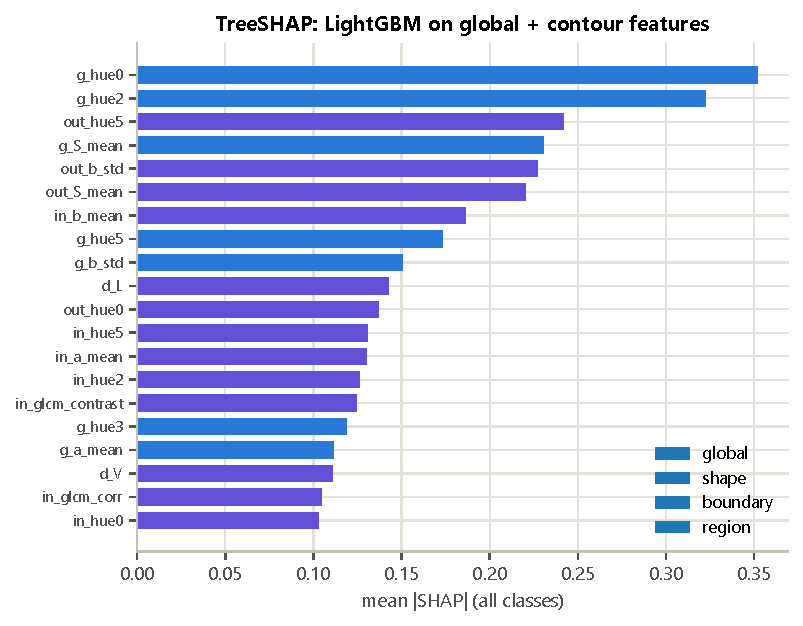
\includegraphics[width=0.7\linewidth]{shap_top20.pdf}
\caption{TreeSHAP importance of the 20 most influential features of the LightGBM model on global and contour features (all classes). Region (inside/outside colour and texture) and global colour features dominate; contour shape and boundary features contribute about \shapShape{} and \shapBoundary{} of the total.}
\end{figure}
\begin{figure}[h]
\centering
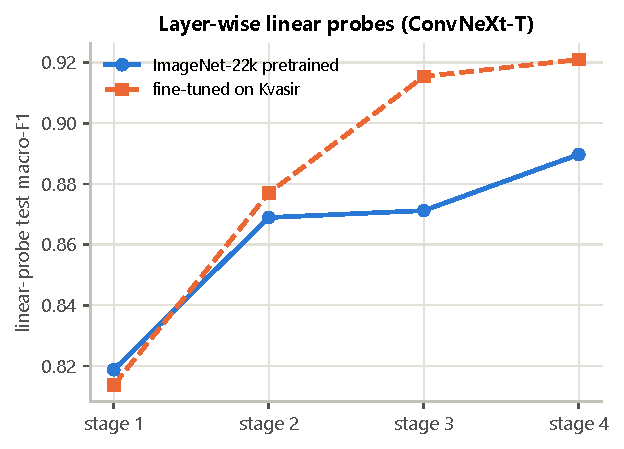
\includegraphics[width=0.55\linewidth]{layerwise_probe.pdf}
\caption{Layer-wise linear probes on ConvNeXt-T stages: ImageNet-22k pretrained versus fine-tuned on Kvasir. Fine-tuning mostly reshapes the last two stages.}
\end{figure}
\begin{figure}[h]
\centering
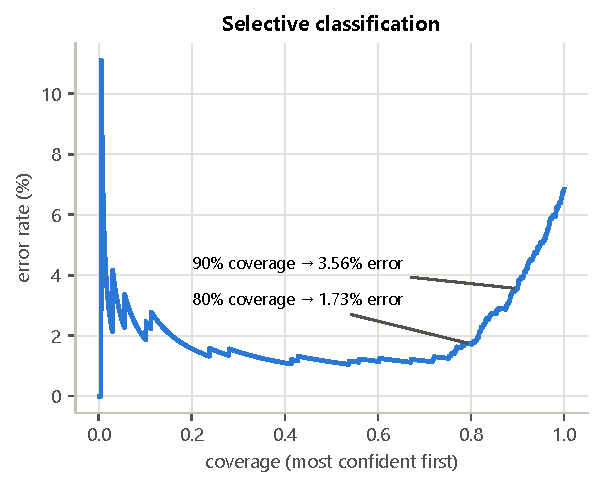
\includegraphics[width=0.5\linewidth]{risk_coverage.pdf}
\caption{Selective classification: error rate on the most confident fraction of test frames (ACG-ConvNeXt, seed 0).}
\end{figure}
\begin{figure}[h]
\centering
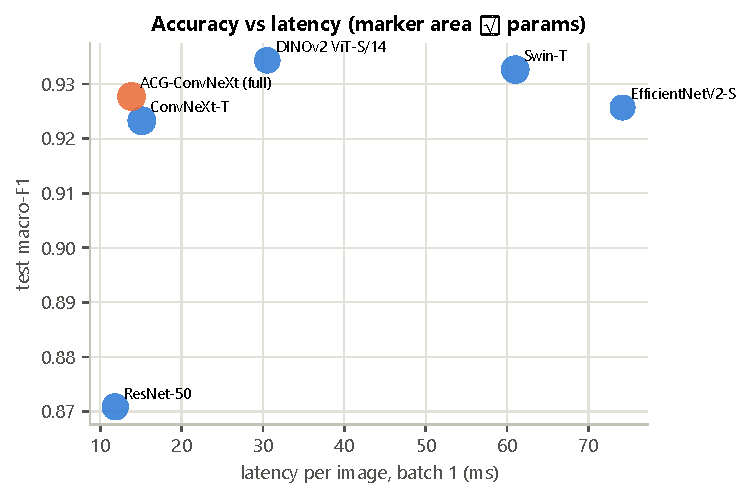
\includegraphics[width=0.55\linewidth]{pareto.pdf}
\caption{Accuracy--latency trade-off (batch-1 latency on an RTX~4060 Laptop GPU; marker area proportional to parameter count).}
\end{figure}
\begin{figure}[h]
\centering
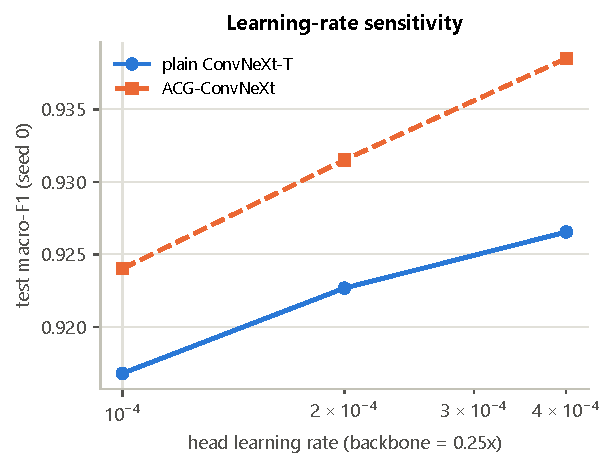
\includegraphics[width=0.5\linewidth]{lr_sensitivity.pdf}
\caption{Learning-rate sensitivity for plain and guided ConvNeXt-T (seed 0). A three-seed replication at twice the default rate is reported in Section~\ref{sec:data} of the results text.}
\end{figure}
\begin{figure}[h]
\centering
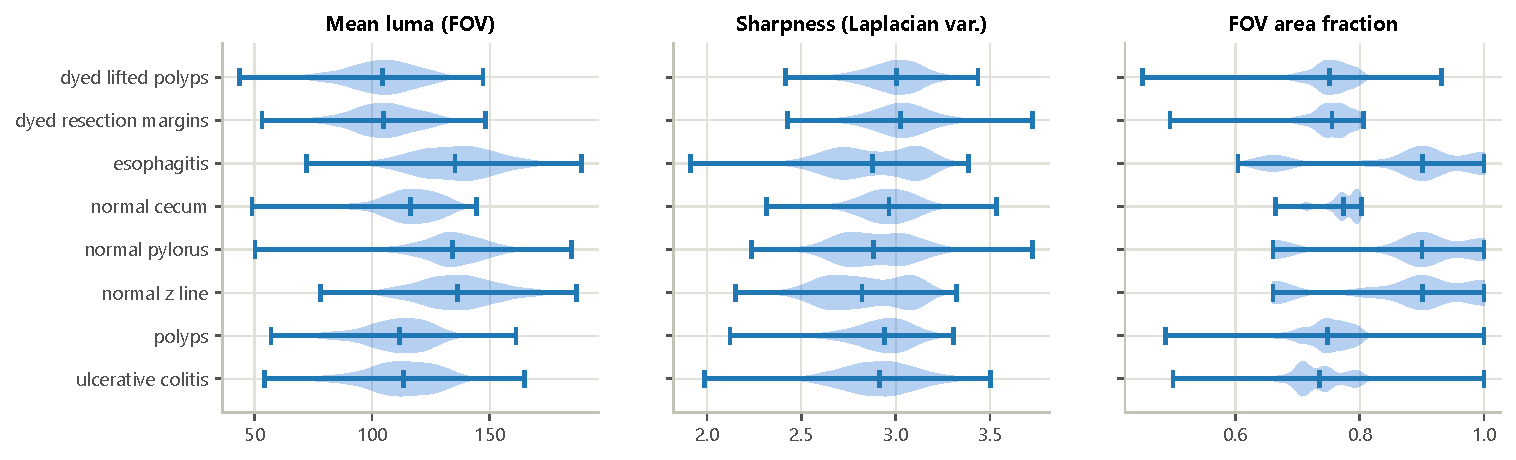
\includegraphics[width=0.9\linewidth]{eda_image_stats.pdf}
\caption{Image statistics by class: mean luma, sharpness and field-of-view fraction.}
\end{figure}
\begin{figure}[h]
\centering
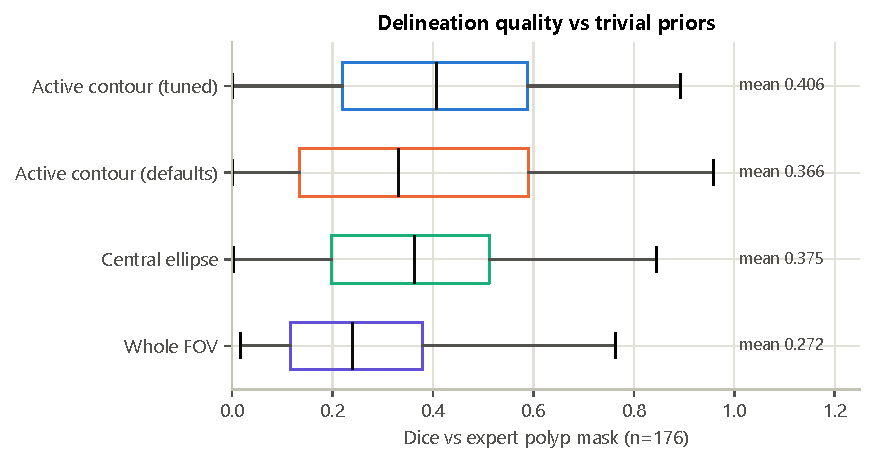
\includegraphics[width=0.6\linewidth]{ac_dice_boxplot.pdf}
\caption{Delineation quality: tuned contour versus trivial priors on 176 expert-masked test-split polyps.}
\end{figure}
